\section{Introduction}
\label{sec:intro}

Creation is not a process that exists in a vacuum but instead relies on and is in conversation with the environment of the artist. Positive inspiration (mimicry and adoption of a similar style) and negative inspiration (contrast with and intentional movement against an established norm) are both integral parts of the process. Although historically the creative process has relied on a high degree of technical knowledge, the development of increasingly sophisticated assistive creative tools has ``democratized" the process by offloading the technical and leaving the creative with the user, who increasingly no longer has to be an artist in the traditional sense. Notably, these tools have been focused on positive inspiration, such as with image analogies and style transfers in general \cite{2001hertzman}.

The rise of neural networks has merely accelerated the growth in this domain with the recent breakthrough of image diffusion for high quality image synthesis \cite{ho2020denoisingdiffusionprobabilisticmodels}. The extension into the time domain has resulted in video diffusion models for video generation \cite{ho2022videodiffusionmodels}.

We propose SAM-IAM, a continuation in this rich tradition of visual media generation, as video synthesis conditioned on an input image and applying motion transfer from an input video. Fundamentally the difference between a static image and a dynamic video is the change in (typically) the subject over time. Extracting the intrinsics of this change and applying it to a static image is in a sense similar to style transfers and analogies, but differs in that the subject is being switched. The process is similar to video diffusion conditioned on an image and text, but is notably more constrained by the input.

However, the problem is still fundamentally underconstrained and ``motion" itself is contextually dependent on both the input and the application. A video of car driving from left to right has the basic left to right motion, but also contains the rotational motion of the wheels. Applying this motion to an image of a motorcycle should preserve the overall left to right motion but also ideally map across the rotation of the wheel. In contrast, applying this motion to an image of a horse should not preserve any rotational
\twocolumn[{%
            \renewcommand\twocolumn[1][]{#1}%
            \centering
            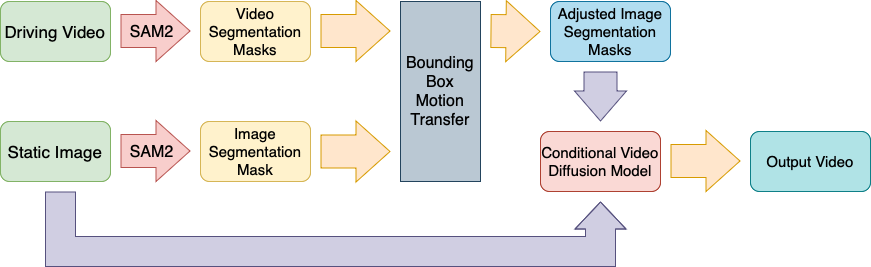
\includegraphics[width=1\linewidth]{media/method.png}
            % \vspace{-2em}
            \captionof{figure}{An overview of our pipeline.}
            \label{fig:method}
        }]
motion. Consequently, ``reasonable" motion transfer becomes highly semantically dependent.

Even ignoring the mapping problems, from a single view, different types of rigid motion are often indistinguishable without context. An object scaling up in size is equivalent to it translating towards the camera. In order to reduce the complexity of the decision space, our work focuses on rigid motion of a single constant foreground object. This careful constraining of the problem allows us to offer a new focus into the overall problem of video synthesis and a novel targeting of scope.
%-------------------------------------------------------------------------

